\documentclass{article}
\usepackage{amsmath}
\usepackage{amssymb}
\usepackage{empheq}
\usepackage{graphicx}
\usepackage{subcaption}
\usepackage{booktabs}
\usepackage{geometry}
\usepackage{mathtools}
\usepackage{bbm}
\usepackage{url}
\geometry{left=2.5cm,right=2.5cm,top=2.5cm,bottom=2.5cm}

\title{\textbf{Lecture Note} \\
		\large CS5339 Theory and Algorithm for Machine Learning}
\author{Meng-Jiun Chiou \\ National University of Singapore \\ mengjiun.chiou@u.nus.edu}

\date{}


\begin{document}
    \maketitle 
    \begin{figure}[h!]
    \centering
    
\includegraphics[width=.8\columnwidth]{Co-Brand-SoC-H}
    \end{figure}
    
    \clearpage
    
    \tableofcontents
    \clearpage
    
    \section{Formulation}
    \subsection{Supervised Learning}
    \subsubsection{Empirical Risk Minimization (ERM)}
    The learner does not know $D$ and only have access to the training set $S$, a sample from $D$. For a predictor $h: X \rightarrow Y$, we can approximate the expected error by using the training set error
    \begin{equation}
    L_S(h) = \frac{|i \in {1,...,m}:h(x_i) \neq y_i|}{m}.
    \end{equation}
    It can be rewritten using the 0-1 loss
    \begin{equation}
    L_S(h) = \frac{\sum_{i=1}^m l_{0-1}(h, (x_i, y_i))}{m}.
    \end{equation}
    Training set error is often called the empirical error or empirical risk. Given a hypothesis class $H$, finding the hypothesis $h \in H$ that minimizes the empirical risk is a simple learning strategy, which is often called empirical risk minimization (ERM).
    
    
    \subsubsection{Maximum Likelihood Estimation (MLE)}
    Assume that the data distribution $P$ is known up to some parameter $h \in H$, MLE selects the $h$ that maximizes the probability of the data $S$ being observed:
    \begin{equation}
    h_{ML} = \arg \max_{h\in H} P(S|h).
    \end{equation}
    For i.i.d. data $S = (z_1,...,z_m) \sim D^m$, this becomes:
    \begin{equation}
    h_{ML} = \arg \max_{h \in H} \prod_{i=1}^m D(z_i | h).
    \end{equation}
    For supervised learning, $z_i = (x_i, y_i)$ and we have
    \begin{align}
    h_{ML} &= \arg \max_{h \in H} \prod_{i=1}^m D(y_i | x_i, h) D(x_i) \\
    	   &= \arg \max_{h \in H} \prod_{i=1}^m D(y_i | x_i, h) \\
           &= \arg \max_{h \in H} \sum_{i=1}^m log D(y_i | x_i, h).
    \end{align}
    With an equivalent distribution can be found, empirical risk minmization (ERM) is equal to maximum likelihood when for loss function
    \begin{equation}
    l(h, (x,y)) = -\ln p(y|x,h).
    \end{equation}
    
    \subsubsection{Classification Loss Functions}
    For binary classification using $h(x) \in (-\infty , \infty)$, we often compose the output of our function $h(x)$ with the logistic (sigmoid) function to get a probability model 
    \begin{align}
    P(y=1|x,h) &= \frac{\exp(h(x))}{1 + \exp(h(x))} = \frac{1}{1+\exp(-h(x))} \\
    P(y=-1|x,h) &= 1-\frac{\exp(h(x))}{1 + exp(h(x))} = \frac{1}{1 + \exp(h(x))}.
    \end{align}
    For $y \in \{1,-1\}$, can write $P(y|x,h) = \frac{1}{1+\exp(-yh(x))}.$ Therefore log loss can be written as
    \begin{equation}
    l_{\log}(h,(x,y)) = -\log P(y|h(x)) = \log(1+\exp (-yh(x))).
    \end{equation}
    When $h(x)$ is a linear function, this is often called \textit{logistic regression}. \\\\
    For multi-class classification, 
    \begin{equation}
    P(y=k|x,h)=\frac{\exp(h_k(x))}{\sum_{i=1}^K \exp (h_i(x))}.
    \end{equation}
    When $h_i(x)$ is linear, it is often called \textit{multiclass logistic regression, softmax regression or maximum entropy classifier}.
    
    \subsubsection{Maximum A Posteriori Estimation (MAPE)}
    Instead of maximizing the likelihood, MAP find the parameter that maximizes the posterior probability $P(h|D)$:
    \begin{align}
    h_{MAP} &= \arg \max_{h \in H} P(h|D) \\
    		&= \arg \max_{h \in H} P(D|h)P(h) \\
            &= \arg \max_{h \in H} \prod_{i=1}^m D(z_i|h)P(h) \\
            &= \arg \max_{h \in H} \sum_{i=1}^m \Big( \log D(y_i|x_i, h) + \log P(h) \Big).
    \end{align}
    So balance between fitting the data (likelihood) and fitting the prior well. For example, we add an zero mean Gaussian prior on the weight vector $\lambda ||\textbf{w}||^2$ in loss function of linear regression. This is often called \textit{ridge regression} or penalized least square. Minimizing a combination of empirical risk and a regularizer is also called Regularized Risk Minimization (RRM).
    
    \subsubsection{Bayesian Estimation}
    Instead of selecting a single $h$, we maintain the posterior distribution over the parameters $P(h|z_1,...,z_m)$. This can be used to make optimal prediction (assuming the prior is correct) for the variable of interest. For example, 
    \begin{align}
    P(y|x,z_1,...,z_m) &= \int_h P(y,h|x,z_1,...,z_m) \\
    				   &= \int_h P(y|h,x,z_1,...,z_m) P(h|z_1,...,z_m).
    \end{align}
    
    
    \subsection{Unsupervised Learning}
    Many (but not all) unsupervised learning problems can be posed as density estimation problems, i.e. learning the distribution of the data. We can also pose the problem of learning the data distribution as a maximum likelihood (or maximum a posteriori) estimation problem. 
    \\\\
    For lossless compression, using $P(x_1,...,x_n)$ to compress $x_1,...,x_n$ using Hoffman coding or arithmetic coding, gives the  shortest code length of $-\sum_{i=1}^m \log P(x_i|h)$ (ignoring rounding required for discrete lengths). Therefore, maximizing $P(x_i|h)$ is equal to minimizing number of bits required.
    
    \subsection{Discriminative/Generative Models}
    The approach of directly optimizing for the loss that we are interested in is called \textbf{discriminative learning}. Another approach is to ignore the fact that the data for supervised learning comes in pairs $z=(x,y)$ and learn the data distribution (density estimation) for $z$. After we have learned a model for $p(z) = p(x,y)$, we perform inference to get our estimate of $y$ by computing $p(y|x)$. This approach is called \textbf{generative learning}. We illustrate this approach using two common learning models: naive Bayes and linear discriminant analysis (LDA).
    
   \subsubsection{Naive Bayes}
   The Bayes optimal classifier is 
   \begin{align}
   h_{Bayes}(x) &= \arg\max_{y \in {-1, 1}} P(Y=y|X=\textbf{x}) \\
   				&= \arg\max_{y \in {-1, 1}} P(Y=y)P(X=\textbf{x}|Y=y)/Z
   \end{align}
   and we make the naive generative assumption that, the features are independent of each other given the label, i.e.
   \begin{equation}
   P(X=\textbf{x}|Y=y) = \prod_{i=1}^d P(X_i=x_i|Y=y).
   \end{equation}
   Hence, the classifier becomes.
   \begin{align}
   h_{Bayes}(x) &= \arg\max_{y \in {-1, 1}} P(Y=y) \prod_{i=1}^d P(X_i=x_i|Y=y) \\
   &= \arg\max_{y \in {-1, 1}} \log P(Y=y) + \sum_{i=1}^d \log P(X_i=x_i|Y=y) \\
   &= sign(w_0 + \sum_{i=1}^d(w_{i,0}x_{i,0}+w{i,1}x{i,1})).
   \end{align}
   There comes a question: which is better, Naive Bayes or logistic regression? An answer \cite{4690} said it depends on the distribution of data. If the data set is large, discriminative model may perform better as it models directly $p(y|x)$. On the other hand, if there are some extra unlabeled data, generative model may do better as it can deal with missing data.
   
   \subsubsection{Linear Discriminant Analysis (LDA)}
   LDA and QDA classifiers are attractive because they have closed-form solutions that can be easily computed, are inherently multiclass, have proven to work well in practice and have no hyperparameters to tune. Linear Discriminant Analysis can only learn linear boundaries, while Quadratic Discriminant Analysis can learn quadratic boundaries and is therefore more flexible..
   
   \subsubsection{Discriminative VS Generative Classifiers}
   Here are some comparisons between these two classes of models. Pros for \textbf{discriminative models}:
   \begin{itemize}
   \item Discriminative classifiers are more robust against misspecification of the model, while generative classifiers depend on the model being correct. If the model is wrong, the discriminative model can still converge to the best approximation within the model class as the data size increases.
   \item It is usually easier to add features to discriminative models. For generative model, we need to try to find the correct model for the feature, which can be difficult.
   \end{itemize}
   Pros for \textbf{generative models}:
   \begin{itemize}
   \item It is sometimes computationally cheaper to train generative classifiers, e.g. Naive Bayes mostly requires only counting.
   \item It may converge faster, e.g. Naive Bayes converges faster than logistic regression.
   \item It handles missing and unlabeled training data naturally. In doing inference, they are marginalized away. However, in discriminative models there is no standard way for handling missing/unlabeled variables.
   \end{itemize}
   
   \subsection{Feature}
   \subsubsection{Filter}
   Asses each feature independently of other features. We may select $k$ features that achieves the highest score, using \textbf{Pearson correlation coefficient}:
   \begin{equation}
   \rho_(X_j, Y) = \frac{cov(X_j, Y)}{\sqrt{var(X_j)var(Y)}} = \frac{cov(X_j, Y)}{\sigma_{X_j} \sigma_{Y}}
   \end{equation}
   For classification, \textbf{mutual information} (MI) is often used. Not limited to real-valued random variables like the correlation coefficient, MI is more general and determines how similar the joint distribution $p(X,Y)$ is to the products of factored marginal distribution $p(X)p(Y)$. MI is defined as:
   \begin{align}
   I(X_i;Y) &= \sum_{x_i} \sum_{y} p(x_i, y) \log \frac{p(x_i, y}{p(x_i)p(y)} \\
   			&= H(Y) - H(Y|X),
   \end{align}
   where $p(x_i,y)$ is the joint probability function of $X$ and $Y$, and $p(x_i)$ and $p(y)$ are the marginal probability distribution functions of $X$ and $Y$ respectively and $H(Y) - H(Y|X)$ is the difference between the entropy of the label $Y$ and the conditional entropy of $Y$ given input $X$ and is also called the \textbf{information gain}. For feature selection, we rank features according to information gain, and select the $k$ features with the largest information gain. Another commonly used feature selection method is \textbf{chi square} which tests whether the feature is independent of the label.
   
   \subsubsection{Wrapper}
   Filter approaches do not take into account dependence among the features. Wrapper approaches search for subset of variables that will perform well. Common greedy methods include:
   \begin{itemize}
   \item Forward selection: Features are progressively added as learning is done. e.g. Viola-Jones face detector is trained using Adaboost.
   \item Backward elimination: Starting with all variables and progressively eliminate the least promising ones.
   \end{itemize}
   
   \subsubsection{Sparsity-Inducing Norms}
   We can formulate the feature selection problem as:
   \begin{equation}
   \min_{w} L_S(\textbf{w}) s.t. ||\textbf{w}||_0 \leq k,
   \end{equation}
   where $||\textbf{w}||_0 = |\{ i:w_i \neq 0 \}|.$ is also called $l0$ norm. As this is often computationally hard, so we often relax into $l1$ norm:
   \begin{equation}
   \min_{w} L_S(\textbf{w}) s.t. ||\textbf{w}||_1 \leq k,
   \end{equation}
   which can be solved efficiently if $L_S$ is convex (convex optimization problem). We can also encourage a sparse solution to use the $l1$ norm of the weight as a regularizer,
   \begin{equation}
   \min_{w} (L_S(\textbf{w}) + \lambda ||\textbf{w}||_1),
   \end{equation}
   which again is convex if $L_S$ is convex, e.g. in logistic regression. 
   \\\\
   We can derive Lasso as MAP with each $w_i$ independently distributed with Laplacian prior $Pr(w_i) = \frac{\lambda}{2}\exp(-\lambda |w_i|)$. Refer to Figure \ref{fig:lasso_ridge}.
   \begin{figure}[h!]
   \centering
   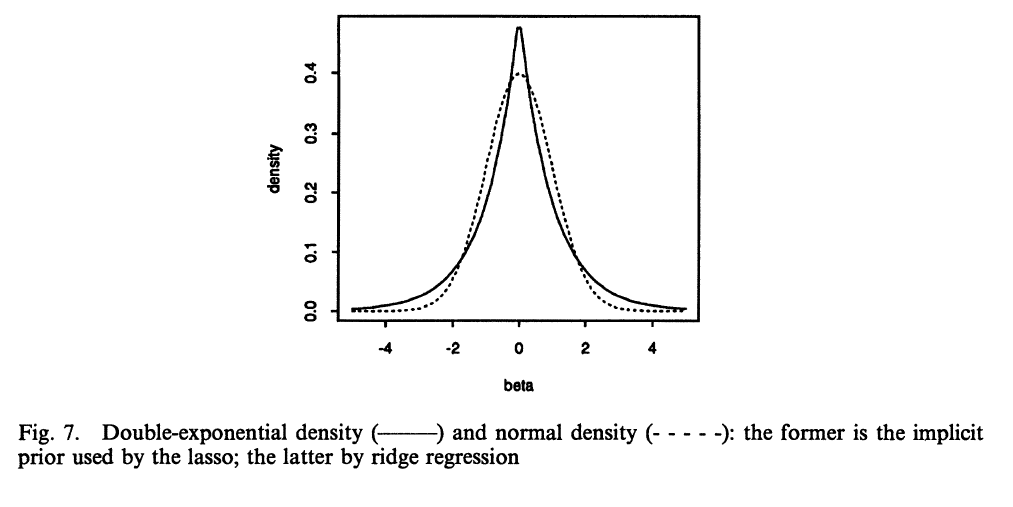
\includegraphics[width=.8\columnwidth]{lasso_ridge}
   \caption{Laplacian prior (l1, double-exponential density) versus Gaussian prior (l2, normal density).}
   \label{fig:lasso_ridge}
   \end{figure}
   Compared to Lasso, Ridge regression performs poor for the data out of range of training data. Lasso regression zeros out most of the coefficients.
   
   \subsubsection{Common Feature Transformation Methods}
   Let $\textbf{f} = (\text{f}_1,...,\text{f}_m) \in \mathbb{R}^m$ be the value of feature f over the $m$ training examples and $\bar{\text{f}} = \frac{1}{m} \sum_{i=1}^m \text{f}_i$.
   \begin{itemize}
   \item Centering
   \item Unit Range
   \item Standardization (zero mean and unit variance)
   \item Clipping
   \item Sigmoidal Transformation
   \item Logarithmic Transformation
   \end{itemize}
   
   \subsubsection{Feature Learning}
   Instead of selecting a subset of predefined features, we can also learn a feature mapping $\varphi : \mathcal{X} \rightarrow \mathbb{R}^d$ which maps instances in $\mathcal{X}$ to $d$ dimensional feature space. If we have a lot of unlabeled data, may be useful to do unsupervised feature learning, called \textbf{dictionary learning}. 
   \\\\
   To do dictionary learning, it is common to construct an autoencoder consisting of a function pair: an encoder $\varphi: \mathbb{R}^d \mapsto \mathbb{R}^k$ and  a decoder $\phi: \mathbb{R}^k \mapsto \mathbb{R}^d$. The goal of learning is to minimize the reconstruction error: $\sum_i || \textbf{x}_i - \phi(\varphi(\textbf{x}_i)) ||^2$. Principal Component Analysis (PCA) is an example where $k < d$.
   
   \section{Representation}
   Some interesting functions can be represented/approximated:
   \begin{itemize}
   \item \textbf{Boolean functions}: arbitrary boolean functions from $\{0,1\}^d$ to $\{0,1\}$.
   \item \textbf{PARITY}: a boolean function from $\{0,1\}^d$ which returns 1 if the number of the occurences of $1$ in the input is odd and returns $0$ otherwise. 
   \item \textbf{Continuous functions}: Functions from $[0,1]^d$ to $\mathbb{R}$ satisfying the property: f is continuous if for any $\epsilon > 0$, there exists a $\delta > 0$ such that for all $\textbf{x},\textbf{x}' \in [0,1]^d$ where $||x-x'||<\delta$, we have $|\text{f(x)}-f(x')|<\epsilon.$
   \item \textbf{Lipschitz functions}: A function f is c-Lipschitz for some $c > 0$ if for all $\textbf{x},\textbf{x}' \in \mathcal{X}$, $|\text{f}(\textbf{x}) - \text{f}(\textbf{x}')| \leq c||\textbf{x}-\textbf{x}'||$.
   \end{itemize}
   We call a function class F a universal approximator if it is able to approximate any continuous function to arbitrary accuracy: for any continuous function f, there is a $g \in F$ such that $\sup_{x\in [0,1]^d} |f(\textbf{x})-g(\textbf{x})|<\epsilon$.
   
   \subsection{Nearest Neighbor (NN)}
   Among the simplest learning algorithm, it simply memorize the training set and predict with the label of the nearest neighbor (NN) in the training set. It requires a distance function to measure the distances. NN can represent any Boolean function -- simply store the label for each possible input. NN is also an universal approximator -- store the value of the function at a fine enough regular grid. NN has some properties:
   \begin{itemize}
   \item NN converges to at most twice the optimal error (Bayes error), as training set size grows.
   \item kNN converges to Bayes error.
   \end{itemize}
   NN suffers curse of dimensionality. (SSBD Theorem 19.3) Let $\mathcal{X}=[0, 1]^d$, $\mathcal{Y} = \{0, 1\}$, and $\mathcal{D}$ be a distribution over $\mathcal{X \times Y}$ for which the conditional probability function, $p(y|x)$ is a c-Lipschitz function. Let $h_S$ denote the result of applying the 1-NN rule to a sample $S \sim \mathcal{D}^m$. Then, 
   \begin{equation}
   E_{S \sim \mathcal{D}^m} [L_D(h_S)] \leq 2L_\mathcal{D}(h^*) + 4c\sqrt{d}m^{-\frac{1}{d+1}},
   \end{equation}
   where $h^*$ is the Bayes decision rule. The first term is optimal error, and the last term represents curse of dimension. For the last term to be smaller than $\sigma$, $m > (4c\sqrt{d}/\epsilon)^{d+1}$ is sufficient. This means sample size grows exponentially with dimension $d$. Some properties:
   \begin{itemize}
   \item It can bound the expected error by twice the optimum plus $c$ times the expected distance of the points from its nearest neighbors.
   \item It cover the space with boxes of sides $\epsilon$.
   \item If point and nearest neighbor fall in the same box, distance at most $\sqrt{d}\epsilon$, otherwise upper bound with largest distance in $[0,1]^d$ which is $\sqrt{d}$.
   \item The probability of nearest neighbor falling into a different box can be bounded by a constant factor of the number of boxes, which is roughly proportional to volume which grows exponentially with dimension.
   \item Balanccing $\epsilon$ with probability gives second term in the bound. 
   \end{itemize}
   SSBD Theorem 19.4 shows that the sample size necessarily grows exponentially with dimension if we only impose the Lipschitz condition. Some other practical properties:
   \begin{itemize}
   \item NN and k-NN suffer from the \textit{curse of dimensionality}.
     \begin{itemize}
     \item If there are irrelevant variables, removing them could be helpful.
     \item Do feature selection.
     \end{itemize}
   \item Scaling/normalization of features important as it affects distance computation.
  	\item As suggested by the Lipschitz constant in performance bound, NN will do well if instances from the same class are clustered close together and the clusters are far from each other. If all tests and final prediction are binary, the function represented by the decision tree can be interpreted as a DNF (disjunction of conjunctions).
   \end{itemize}
   
   
   \subsection{Decision Tree}
   In a decision tree, the leaves are labeled with the class while each internal node contains a test(usually on a single variable). To do classification, we start from the root node and perform the test at the node, move to the child corresponding to the test output, and recurse until we reach a leaf node, which gives the class of the instance.
   \\\\
   For Boolean functions, it is useful to understand properties of decision trees in relation to standard Boolean formulation.
   \begin{itemize}
   \item \textbf{Disjunctive Normal Form (DNF)}: Disjunction (OR) of conjunctions (AND) of variables or their negations, e.g. $(x_1 \wedge \neg x_3 \wedge x_4) \vee ... \vee (x_2 \wedge x_5 \wedge \neg x_8)$.
   \begin{itemize}
   	\item \textbf{$\mathbf{k}$-term DNF}: when the number of conjunctive terms is no more than $k$.
    \item \textbf{$\mathbf{k}$-DNF}: when the number of literals (variables or its negation), also called width, is no more than $k$.
   \end{itemize}
   
   \item \textbf{Conjunctive Normal Form (CNF)}: Conjunction (AND) of disjunctions (OR) of variables or their negations, e.g. $(x_2 \vee \neg x_5) \wedge ... \wedge (\neg x_4 \vee x_6 \vee x_9)$.
   \begin{itemize}
   \item \textbf{$\mathbf{k}$-clause CNF}: when the number of disjunctive clauses is no more than $k$.
   \item \textbf{$\mathbf{k}$-CNF}: when the number of literals, or width, is no more than $k$.
   \end{itemize}
   \end{itemize}
   A decision tree representation of a boolean function with $k$ leaves can be represented with a \textbf{$\mathbf{k}$-term DNF}. There are at most $k$ leaves with label 1. Represent each leaf as the conjunction of the literals representing the path from the root. Take the disjunction of the terms. Furthermore, a depth $d$ decision tree can be represented as a \textbf{$\mathbf{d}$-DNF}. On the other hand, a binary decision tree with $k$ leaves can also be represented with a \textbf{$\mathbf{k}$-clause CNF}, by representing each leaf as the conjunction of the literals representing the path to the leaves with label 0 from the root. A depth $d$ decision tree can also be represented as a \textbf{$\mathbf{d}$-CNF} -- the tree depth corresponds to the width of the formula.
   \\\\
   Trees are \textbf{universal approximators}, since it can 
   \begin{itemize}
   \item represent any Boolean function
   \item approximate any continuous function
   \end{itemize}
   However, to represent PARITY and DISTINCT: $\{0,1\}^{2d} \rightarrow \{0,1\}$, it requires $2^d$ leaves: exponential in the number of inputs. \textbf{Restricting the rules tot take the form of a tree instead of disjunctions of them sometimes result in requiring an exponentially larger representation}.
   \\\\
   Some practical properties of trees:
   \begin{itemize}
   \item Trees are usually more interpretable to humans
   \item Features do not need to be scaled/normalized.
   \item However, it can be unstable: small change in training data can result in large change in the learned tree.
   \item Often does not generalize as well as other learning methods
   \item But can use with ensemble methods to provide learning methods that scale well and generalize well -- ensembles are able to represent unions, intersections and other functions of the base classes.
   \begin{itemize}
   \item Multiple trees are trained with random subsets of the training example to obtain a \textit{random forest} and then output a combination of the outputs of the trees.
   \item Weighted combinations of trees, often trained using boosting techniques also performs well.
   \end{itemize}
   \end{itemize}
   
   \subsection{Linear Predictors}
   Given input $\textbf{x} = (x_1,...,x_d) \in \mathbb{R}^d$, a linear function, parameterized by a weight vector $\textbf{w} = (w_1,...w_d),$ is defined as
   \begin{equation}
   f(\textbf{x}) = \textbf{w}^T \textbf{x} = \sum_{i=1}^d w_i x_i.
   \end{equation}
   A linear function is necessarily zero when \textbf{x} is the zero vector. An affine function has an offset $b$, often called the bias:
   \begin{equation}
   f(\textbf{x}) = \textbf{w}^T \textbf{x} + b = \sum_{i=1}^d w_i x_i + b = \sum_{i=0}^d w_i x_i. \ \ (\text{set}\ w_0 = 0)
   \end{equation}
   Linear functions are often used for regression giving linear regression.
   \\\\
   We can also use a linear function as a classifier by composing it with the sign function, which is also called \textit{linear threshold function}:
   \begin{equation}
   f(\textbf{x}) = sign(\textbf{w}^T \textbf{x} + b) = 
   		\begin{cases}
   		1\ \ \text{if}\ \sum_{i=1}^d w_i x_i \geq -b\\
        0\ \ \text{otherwise}
   		\end{cases}.
   \end{equation}
   where $-b$ is the threshold. Positive region is often called halfspace. We call the function class \textit{homogeneous halfspaces} when threshold zero and \textit{nonhomogeneous halfspaces} when threshold nonzero.
   
   \subsection{Support Vector Machine}
   \subsubsection{Margin and Hard SVM}
   Let $S = (x_1, y_1),...,(x_m, y_m)$, where $x_i \in \mathbb{R}^d$ and $y_i \in \{-1,1\}$. The training set is separable if there exists $(\textbf{w},b)$ such that $y_i = \text{sign}(\langle \textbf{w}, x_i \rangle + b)$ for all $i$. That is, $\forall i \in [m],\ y_i(\langle \textbf{w}, x_i \rangle + b) > 0.$ Hard SVM returns the hyperplane that separates the points with the largest possible margin.
   \\\\
   (SSBD Claim 15.1) The distance between a point $\mathbf{x}$ and the hyperplane defined by $(\mathbf{w}, b)$ where $||\mathbf{w}|| = 1$ is $|\langle \mathbf{w}, \mathbf{x} \rangle + b|$. Therefore, we can transform the problem of maximizing distance to that of maximizing the magnitude of the output subject to $||\mathbf{w}|| = 1$. The smallest magnitude on the data points subject to $||\mathbf{w}|| = 1$ is called the \textbf{margin}. Hence, when the problem is separable ($\forall i, y_i(\langle \textbf{w}, x_i \rangle + b) > 0$), hard SVM solves for
   \begin{equation}
   \mathop{\arg \max}_{(\mathbf{w},b):||\mathbf{w}||=1} \min_{i \in [m]} y_i(\langle \textbf{w}, x_i \rangle + b).
   \end{equation}
   We can turn the hard SVM problem into a quadratic optimization problem using the following lemma:
   \begin{equation}
   (w_0, b_0) = \mathop{\arg \min}_{(\mathbf{w}, b)} ||\mathbf{w}||^2\ \ \text{s.t.}\  \forall i, y_i(\langle \textbf{w}, x_i \rangle + b) \geq 1.
   \end{equation}
   Then $(\hat{\mathbf{w}}, \hat{b})$ where $\hat{\mathbf{w}} = \frac{\mathbf{w}_0}{||\mathbf{w}_0||}$ and $\hat{b} = \frac{b_0}{||\mathbf{w}_0||}$ is a solution to the hard SVM problem. \\
   
   \begin{figure}
   \centering
   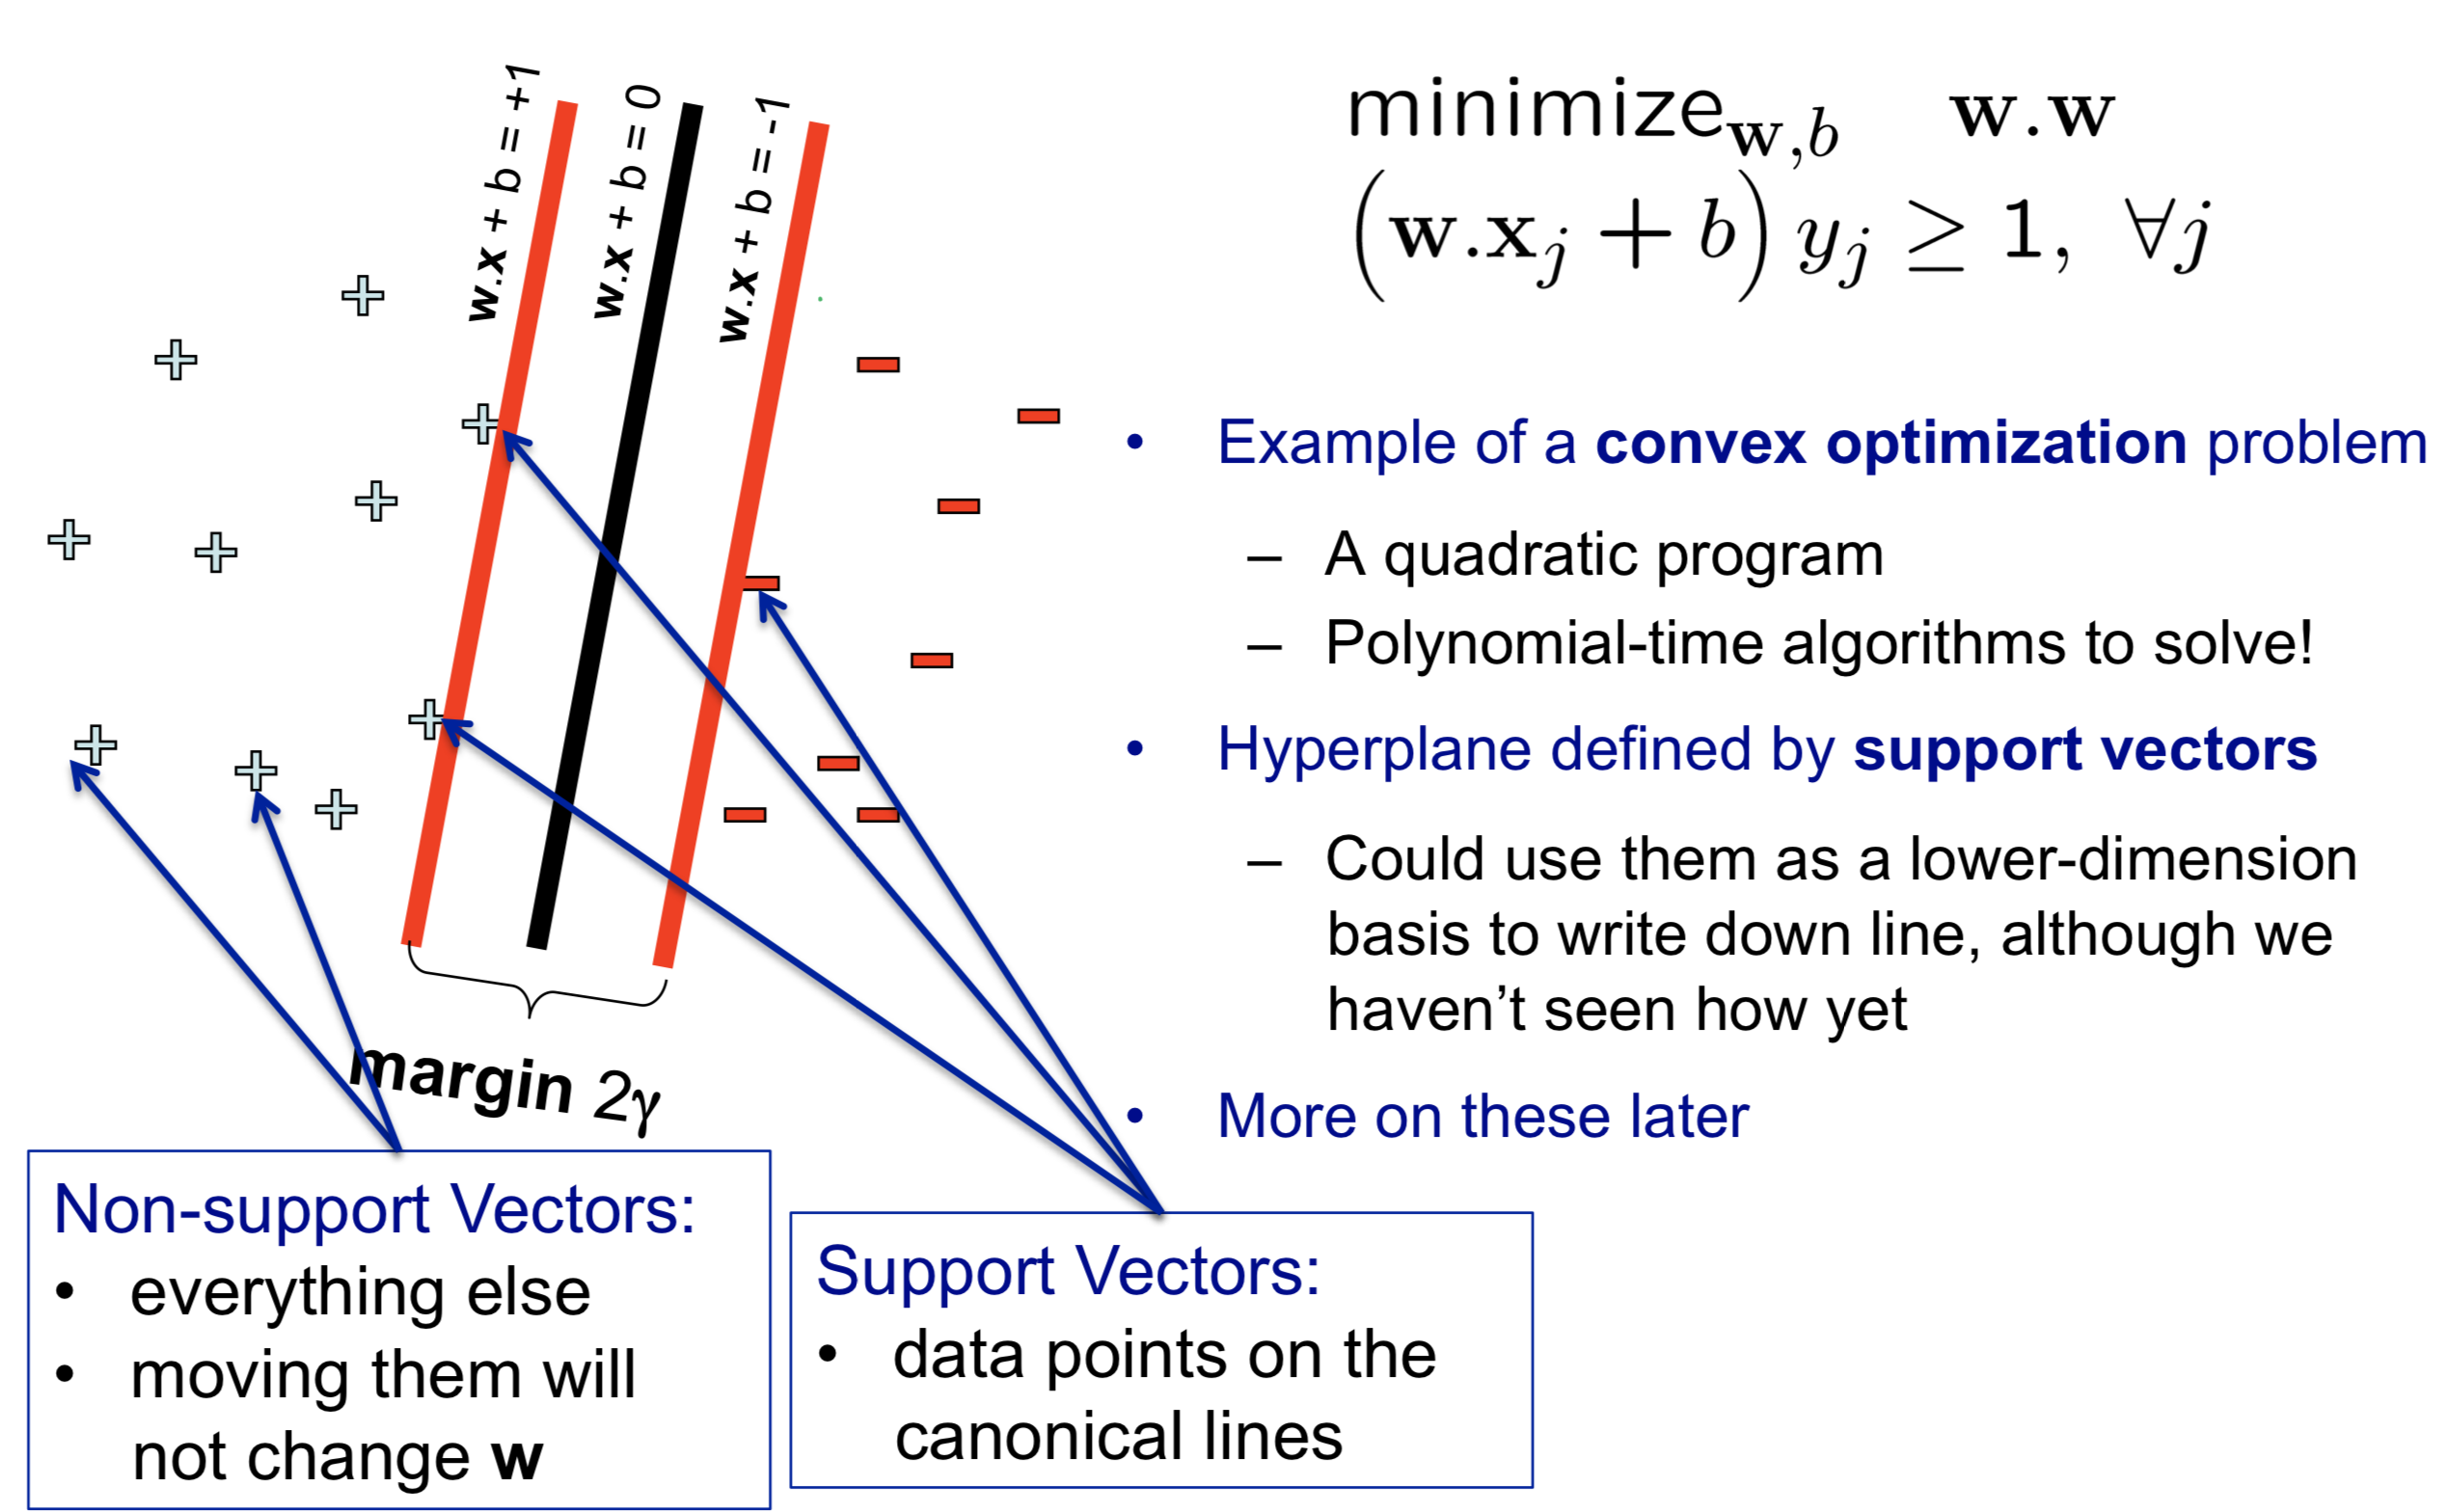
\includegraphics[width=.8\linewidth]{hard_svm}
   \caption{Hard SVM explained.}
   \end{figure}
   
   Soft SVM relaxes the hard constraints for all $i$ in order to handle non-separable cases. This is done by introducing slack variables $\xi_1...\xi_m$ which replace the constraints with $y_i(\langle \textbf{w}, x_i \rangle + b) \geq 1 - \xi_i$. The slack variables $\xi_i$ measure how much the constraints are being violated. We want the slack variables to be small. This leads to optimize
   \begin{equation}
   \min_{\mathbf{w}, b, \mathbf{\xi}} \Bigg( \lambda ||\mathbf{w}^2|| + \frac{1}{m} \sum_{i=1}^m \xi_i \Bigg) \ \ 
   \text{s.t.} \ \forall i, y_i(\langle \textbf{w}, x_i \rangle + b) \geq 1 - \xi_i\ \text{and}\ \xi_i \geq 0.
   \end{equation}
   The hinge loss is defined as $\ell^{hinge} (y, \hat{y}) = \max \{ 0, 1-y_i(\langle \textbf{w}, x_i \rangle + b) \}$, and is denoted as $L_S^{hinge}(y,\hat{y})$. The soft SVM becomes a regularized loss minimization problem:
   \begin{equation}
   \min_{\mathbf{w},b} \Bigg( \lambda||\mathbf{w}||^2 + L_S^{hinge}(y, (\mathbf{w}, b)) \Bigg)
   \end{equation}
   The solution of hard SVM, $\mathbf{w}_0$ is supported by (i.e. in the span of) the examples that are exactly at distance $\frac{1}{||\mathbf{w}_0||}$ from the separating hyperplane.
   \\\\
   (SSBD Theorem 15.8) For hard SVM
   \begin{equation}
   (w_0, b_0) = \mathop{\arg \min}_{(\mathbf{w}, b)} ||\mathbf{w}||^2\ \ \text{s.t.}\  \forall i, y_i(\langle \textbf{w}, x_i \rangle + b) \geq 1,
   \end{equation}
   and let $I = \{ i:|\langle \mathbf{w}_0, \mathbf{x}\rangle| + b_0 = 1 \}$ there exists coefficients $\alpha_1,...,\alpha_m$ such that $w_0 = \sum_{i \in I} \alpha_i \mathbf{x}_i$.
   
   \subsubsection{Representation Power of Linear Threshold Functions}
   What are the boolean functions representable by the linear threshold function?
   \begin{itemize}
   \item AND function
   \item OR function
   \item NOT function
   \end{itemize}
   XOR (PARITY function), however, can not be represented by halfspaces. More generally, if the probability of the positive class does not change monotonically with the value of each input, then linear classifier may not be suitable.
   
   \subsubsection{How many functions can a linear threshold function represent?}
   More generally, how many functions can a hypothesis class $\mathcal{H}$ represent on an arbitrary set of $m$ input points $c_1,...,c_m$?
   \begin{itemize}
   \item VC dimension
   \item Growth function
   \item Shattering
   \item Sauer's lemma
   \end{itemize}
   Refer to slide \textit{Representation I}.
   
   \subsection{Linear combination of Functions}
   The XOR that cannot be represented by a linear classifier can be represented by a thresholded quadratic function, which can represent an ellipse.
   \begin{equation}
   f(x_1, x_2) = \text{sign}(b+w_1x_1+w_2x_2+w_3x_1x_2+w_4x_1^2+w_5x_2^2).
   \end{equation}
   The quadratic function, or more generally polynomial functions, can also be viewed as a linear combination of features. In this case, the features are the monomials $(x_1, x_2, x_1x_2, x_1^2, x_2^2)$. A feature is just a function of the input, e.g. $g_1(x_1, x_2) = x_1,...,g_5(x_1,x_2)=x_2^2$ are the features in this example. 
   \\\\
   Linear combination of functions is very commonly used in machine learning:
   \begin{itemize}
   \item Kernel methods
   \item Single hidden layer neural networks
   \item Matrix/tensor factorization
   \item Ensemble methods
   \end{itemize}
   
   \subsection{Kernel Method}
   Previously, XOR has been showed that it cannot be represented by a linear threshold function but can be represented by a threshold quadratic function:
   \begin{equation}
   f(x_1, x_2) = \text{sign} (b+w_1x_1+w_2x_2+w_3x_1x_2+w_4x_1^2+w_5x_2^2).
   \end{equation}
   We can construct a mapping $\psi : \mathbb{R}^2 \rightarrow \mathbb{R}^5$ as
   \begin{equation}
   \psi (x_1, x_2) = (x1, x2, x_1x_2, x_1^2, x_2^2).
   \end{equation}
   Then we have a linear function in the feature space:
   \begin{equation}
   f(x_1, x_2) = \text{sign} (b+\mathbf{w}^T\psi(x_1, x_2)).
   \end{equation}
   In high dimensions, the number of monomials in a polynomial grows exponentially with degree, so polynomials that contains all monomials cannot be computed efficiently in high dimensions. We use the kernel trick to avoid having to compute the value of each feature. 
   \\\\
   \textit{Kernel} refers to a function that computes the inner product between two elements in the feature space. Given an embedding $\psi$ of the domain space $\mathcal{X}$ into some Hilbert space, we define the kernel function $K(x, x') = \langle \psi(\mathbf{x}), \psi(\mathbf{x}') \rangle$. We use kernels that can be efficiently computed so that inner products in high or even infinite dimensional feature spaces can be efficiently computed.
   \begin{itemize}
   \item The $d$-th Polynomial kernel: $K(\mathbf{x}, \mathbf{x}') = (1+\langle \mathbf{x}, \mathbf{x}' \rangle )^d$.
   \item Gaussian (RBF) Kernel on $\mathcal{R}$: $K(\mathbf{x}, \mathbf{x}') = e^{-\frac{||x-x'||^2}{2\sigma}}$.
   \end{itemize}
   Generally, a function k(x,y) is a valid kernel function (in the sense of the kernel trick) if it satisfies two key properties:
   \begin{itemize}
   \item symmetry: $k(x,y)=k(y,x)$
   \item positive semi-definiteness.
   \end{itemize}
   From the experiment, we know non-linear kernel is helpful for handwritten digit problem.
   
   \subsubsection{Hilbert Space}
   Given a mapping $\psi$ that maps to a finite feature space, we can then compute inner product and distances in the feature space like we do in $\mathbb{R}^d$. But what if the mapping $\psi$ maps the instances to infinite length feature vectors? We would like to extend the notion of $\mathbb{R}^d$ to infinite dimensional vector and even function spaces: Hilbert spaces.
   \\\\
   Some properties we need to define Hilbert Space: 
   \begin{itemize}
   \item The norm of an element is $||v||=\sqrt{\langle v, v \rangle}$.
   \item The distance between two elements is defined in terms of the norm: $d(u,v)=||w-v||=\sqrt{\langle u-v, u-v \rangle}$.
   \item The inner product allows us to define orthogonality: $u$ and $v$ are orthogonal if $\langle u, v \rangle = 0$.
   \item Cauchy-Schwarz inequality: $|\langle u,v \rangle| \leq ||u|| ||v||$.
   \item A Hilbert space $\mathcal{H}$ is complete inner product space, i.e. every Cauchy sequence converges to a point in $\mathcal{H}$.
   \end{itemize}

	\subsubsection{Representer Theorem}
    The representer theorem shows how to use inner products for solving many learning tasks.
    \\\\
    \textbf{Representer Theorem}. Let $\psi$ be a mapping from $\mathcal{X}$ to a Hilbert space. Then there exists a vector $\alpha \in \mathbb{R}^m$ such that $\mathbf{w} = \sum_{i=1}^m \alpha_i \psi(x_i)$ is an optimal solution to
    \begin{equation}
    \min_{\mathbf{w}} \Big( f(\langle \mathbf{w}, \psi(\mathbf{x}_1) \rangle,...,\langle \mathbf{w}, \psi(\mathbf{x}_1) \rangle ) + R||w|| \Big),
    \label{rep}
    \end{equation}
    where $f:\mathbb{R}^m \rightarrow \mathbb{R}$ is an arbitrary function and $R:\mathbb{R}_+ \rightarrow \mathbb{R}$ is a monotonically nondecreasing function. The inner product can be written as
    \begin{align}
    \langle \mathbf{w}, \psi(\mathbf{x}_i) \rangle &= \Bigg\langle \sum_{j=1}^m \alpha_j \psi(\mathbf{x}_j), \psi(\mathbf{x}_i) \Bigg\rangle \\
    &= \sum_{j=1}^m \langle \alpha_j \psi(\mathbf{x}_j), \psi(\mathbf{x}_i) \rangle \\
    &= \sum_{j=1}^m \alpha_j K(\mathbf{x}_j, \mathbf{x}_i).
    \end{align}
    Computing the value of a linear function is just taking the inner product between the weight vector and the input features. In the hilbert space, the squared norm is 
    \begin{align}
    ||\mathbf{w}||^2 &= \langle \mathbf{w},\mathbf{w} \rangle = \Bigg\langle \sum_{i=1}^m \alpha_i \psi(\mathbf{x}_i), \sum_{j=1}^m \alpha_j \psi(\mathbf{x}_j) \Bigg\rangle \\
    &= \sum_{i, j=1}^m \langle \psi(\mathbf{x}_i), \psi(\mathbf{x}_j) \rangle = \sum_{i,j=1}^m \alpha_i \alpha_j K(\mathbf{x}_i, \mathbf{x}_j).
    \end{align}
    Therefore, instead of optimizing equation (\ref{rep}), we can optimize
    \begin{equation}
    f\Bigg( \sum_{j=1}^m \alpha_j K(\mathbf{x}_j, \mathbf{x}_1),.., \sum_{j=1}^m \alpha_j K(\mathbf{x}_j, \mathbf{x}_m) \Bigg) + R \Bigg( \sqrt{\sum_{i,j=1}^m \alpha_i \alpha_j K(\mathbf{x}_i, \mathbf{x}_j)} \Bigg).
    \end{equation}
    with respect to the $\alpha_j$'s instead of $\mathbf{w}$. ($m$ dimensional instead of very large (or infinite) dimensional).
    For example, belows are examples of utilizing kernel methods to convert the objective function:
    \begin{itemize}
    \item Soft SVM
    \begin{equation}
    \sum_{i=1}^m \max \Bigg\{ 0, 1-y_i \Bigg( \sum_{j=1}^m \alpha_j K(\mathbf{x}_j, \mathbf{x}_i) \Bigg) \Bigg\} + \lambda \sum_{i,j=1}^m \alpha_i \alpha_j K(\mathbf{x}_i, \mathbf{x}_j)
    \end{equation}
    \item Regularized logistic regression
    \begin{equation}
    \sum_{i=1}^m \log \Bigg\{ 1+y_i \Bigg( \sum_{j=1}^m \alpha_j K(\mathbf{x}_j, \mathbf{x}_i) \Bigg) \Bigg\} + \lambda \sum_{i,j=1}^m \alpha_i \alpha_j K(\mathbf{x}_i, \mathbf{x}_j)
    \end{equation}
    \item ridge regression
    \begin{equation}
    \sum_{i=1}^m \Bigg(y_i - \sum_{j=1}^m \alpha_j K(\mathbf{x}_j, \mathbf{x}_i) \Bigg)^2 + \lambda \sum_{i,j=1}^m \alpha_i \alpha_j K(\mathbf{x}_i, \mathbf{x}_j)
    \end{equation}
    \end{itemize}
    Often the objective function is convex, e.g. in the three cases, allowing efficient learning. We only need to know the value of the $m \times m$ matrix $G$ such that $G_{i,j} = K(\mathbf{x}_i, \mathbf{x}_j)$, often called the Gram matrix for solving these problems, e.g. soft SVM can be written as
    \begin{equation}
    \min_{\alpha \in \mathbb{R}^m} \Bigg( \lambda \mathbf{\alpha}^T G \mathbf{\alpha} + \frac{1}{m} \sum_{i=1}^m \max \{ 0, 1-y_i(G \mathbf{\alpha})_i \} \Bigg),
    \end{equation}
   where $(G\alpha)_i$ is the $i$-th element of the vector obtainned from nultiplying $G$ with $\mathbf{\alpha}$.
   \\\\
   Some representation properties of kernel method:
   \begin{itemize}
   \item With the use of kernel, many techniques for linear functions carry over to non-linear functions, e.g. polynomials.
   \item Certain kernels give rise to universal approximators. In particular, the Gaussian kernel $K(\mathbf{x}, \mathbf{x}') = e^{-\frac{||x-x'||^2}{2\sigma}}$.
   \item Useful for moderate sized datasets. As computing kernels for all pairs grows quadratically, need further approximation techniques to scale to very large datasets.
   \end{itemize}
   
   \subsubsection{Characterizing Kernel Functions}
   We have seen how we construct a kernel by constructing a mapping to feature space, then defining the kernel as the inner product between features. Assume we are given a similarity functino of the form $K:\mathcal{X} \times \mathcal{X} \rightarrow \mathbb{R}$. When is it a kernel, i.e. represents an inner product between $\psi(\mathbf{x})$ and $\psi(\mathbf{x}')$ for some feature mapping $\psi$? 
   \\\\
   \textbf{Positive semidefinite matrix.} A $n \times n$ matrix $A$ is positive semidefinite if $\mathbf{x}^TA\mathbf{x} \geq 0$ for every nonzero vector $\mathbf{x}$.
   \\\\
   \textbf{Gram matrix}. Given $m$ data points $\mathbf{x}_1,...,\mathbf{x}_m$, the $m \times m$ matrix $G$, where $G_{i,j} = K(\mathbf{x}_i, \mathbf{x}_j)$ is called \textit{Gram matrix}.
   \\\\
   \textbf{Lemma.} A symmetric function $K:\mathcal{X} \times \mathcal{X} \rightarrow \mathbb{R}$ implements an inner product in some Hilbert space if and only if it is positive semidefinite; i.e. for all $\mathbf{x}_1,...,\mathbf{x}_m$, the Gram matrix $G_{i,j} = K(\mathbf{x}_i, \mathbf{x}_j)$ is a positive semidefinite matrix.
   \\\\
   The following properties allow valid kernels to be constructed from other valid kernels:
   \begin{itemize}
   \item If $k_1, k_2$ are kernels, $\alpha_1 k_1 + \alpha_2 k_2$ is a kernel for $\alpha_1, \alpha_2 \geq 0$.
   \item If $k_1, k_2$ are kernels, $(k_1, k_2)(x, x') = k_1(x, x')k_2(x, x')$ is also a kernel.
   \item For any mapping $h:\mathcal{X} \rightarrow \mathcal{X}$ and kernel $k_1$, $k(x, x') = k_1(h(x), h(x'))$ is a kernel.
   \item If $g$ is a polynomial with positive coefficients and $k_1$ is a kernel, $k(x, x') = g(k_1(x,x'))$ is a kernel.
   \item If $k_1$ is a kernel, $k(x, x') = \exp (k_1(x,x'))$ is a kernel.
   \end{itemize}
   
   \subsection{Neural Networks}
   Instead of fixed features, it is also natural to parameterize the features and learn the parameters. This can be represented as a single hidden layer neural network. 
   
   \begin{figure}[h!]
   \centering
   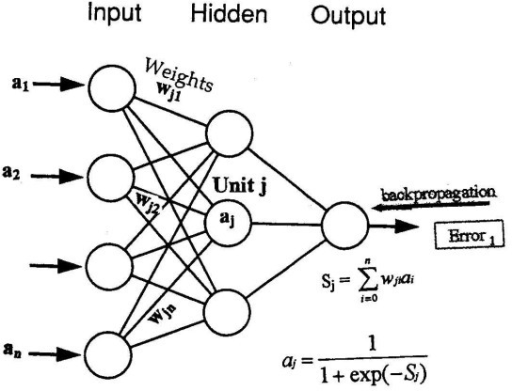
\includegraphics[width=.6\linewidth]{nn}
   \caption{Single hidden layer neural network.} 
   \end{figure} 
   
   \noindent The functions are usually represented in the form $f(\mathbf{x}) = b+ \sum_{i=1}^d w_i \sigma(\mathbf{v}_i^T\mathbf{x})$, where $\sigma(\mathbf{v}_i^T\mathbf{x})$ is called a hidden unit and $\sigma(\cdot)$ is called an activation function. If the output of the hidden unit depends only on the distance to a center $\phi(||\mathbf{x}-c||)$, where $c$ is a parameter, it is often called a \textit{radial basis function}. One common radial basis function is a Gaussian $\phi(||\mathbf{x}-c||) = \exp(\beta ||\mathbf{x}-c||^2)$.
   \\\\
   Commonly used functions for hidden units include:
   \begin{itemize}
   \item Linear threshold function: $\sigma(\mathbf{x},\mathbf{v}) = \text{step}(\mathbf{v}^T\mathbf{x}+\mathbf{v}_0)$.
   \item Linear functions composed with sigmoid $\sigma(\mathbf{x},\mathbf{v}) = \frac{1}{1+e^{-(\mathbf{v}^T\mathbf{x}+\mathbf{v}_0)}}$ or tanh function: $\sigma(\mathbf{x},\mathbf{v}) = \text{tanh}(\mathbf{v}^T\mathbf{x}+\mathbf{v}_0)$. 
   \item Rectifier linear function: $\sigma(\mathbf{x},\mathbf{v}) = \max (0, \mathbf{v}^T\mathbf{x}+\mathbf{v}_0)$.
   \end{itemize}
   
   \subsubsection{Representing All Boolean Functions}
   For the case of using linear threshold activation and considering networks consisting of only AND, OR and NOT gates. A single hidden layer network is sufficient to represent all functions:
   \begin{itemize}
   \item Disjunctive Normal Form (DNF): an OR gate as output with AND gates as the first hidden layer.
   \item Conjunctive Normal Form (CNF): an AND gate as output with OR gates as the first hidden layer.
   \end{itemize}
   As a linear threshold unit can represent AND and OR gates, a single hidden layer neural network with linear threshold units can represent all Boolean functions as well (with negated inputs added).
   
   \subsubsection{Representing PARITY}
   It is know that constant depth circuits (DNF, CNF) using AND, OR and NOT gates requires size exponential in the input dimension $d$ to represent PARITY. The following theorem show that allowing a more powerful linear threshold unit representation can reduce the size to lienar in $d$.
   \\\\
   \textbf{Theorem}: A single hidden layer neural network with linear threshold hidden and output units can represent the PARITY function using $d+1$ hidden units.
   \\\\
   To represent the parity function, we simply set the second layer weights of $\mathbbm{1}_k$ to 1 when $k$ is odd and to $-1$ when $k$ is even, for $0 \leq k \leq d$. The threshold for the output unit is set to $-0.5$.
   \\\\
   To represent PARITY in $d$ dimension using Gaussian kernels with centers fixed at $\{0, 1\}^d$, $2^d - 1$ non-zero coefficients are required. If the centers of the Gaussians and the bandwidth $\sigma$ can be optimized, can represent PARITY using $d+1$ Gaussians.
   
   \subsubsection{Approximating Real-valued Functions}
   A single hidden layer neural network is universal approximator under fairly mild conditions. The sigmoid function can approximate the linear threshold function to arbitrary accuracy by using large enough weights. For more detail, refer to page 52-54, \textit{Representation II}.
   
   \subsubsection{Summary of Representational Properties}
   \begin{itemize}
   \item Single hidden layer neural networks are universal approximators for many types of hidden units.
   \item When the hidden units are learnable, exponential gains in size of representation is sometimes achieved, compared to fixed features.
   \end{itemize}
   
   \subsubsection{Single Hidden Layer NN In Practice}
   \begin{itemize}
   \item Reasonable method when non-linear classifier/regressor required.
   \item Optimization is non-convex, so may depend on initialization. Harder to tune compared to kernel methods.
   \end{itemize}
   For other details, refer to page 57, \textit{Representation II}.
   
   \subsection{Matrix/Tensor Factorization}
   In this section, we switch to unsupervised learning to learn features from unlabeled data. We will look at dimension reduction, which can help supervised learning methods that are sensitive to irrelevant features. Unsupervised learning can also bring in information from large amounts of unlabeled data to help supervised learning when the amount of labeled data is small.
   
   \subsubsection{Principal Component Analysis (PCA)}
   Consider an autoencoder with a function pair: an encoder $\psi:\mathbb{R}^d \mapsto \mathbb{R}^k$ to compress the information and a decoder $\phi:\mathbb{R}^k \mapsto \mathbb{R}^d$ to reconstruct the data from the compressed representation. In PCA, both $\psi(\mathbf{x})=V_k^T \mathbf{x}$ and $\phi(\mathbf{u}) = V_k \mathbf{u}$ are linear transformations. The aim is to minimize the reconstruction error: 
   \begin{equation}
   \min_{\psi, \phi} \sum_i || \mathbf{x}_i - \phi(\psi(\mathbf{x}_i)) ||^2.
   \end{equation}
   Consider the data as a $m \times d$ matrix $X$ where each row represents a data point and each column represents the values of an input dimension. X is firstly normalized (zero mean and unit variance), then be conducted SVD to become $X = U \Sigma V^T$, where the columns of $U$ are the eigenvectors of $XX^T$ and the columns of V are the eigenvectors of $X^TX$. $\Sigma$ is a diagonal $m \times d$ matrix with each entry $\sigma_i$ is called the singular values of $X$ in descending order. 
   \begin{itemize}
   \item $X_k = U_k \Sigma_k V_k^T$ gives the best rank $k$ approximation of $X$.
   \item $XV = U\Sigma$ gives the projection of the data on the principle axes $V$, called the principle components.
   \item $F=XV_k$ is a $m \times k$ matrix that gives the first $k$ principle components for each of the data points. 
   \item (Whitening) We normalize each principle component (feature) to have same variance by $U = XV_k\Sigma^{-1}$.
   \end{itemize}
   
   \subsubsection{Latent Semantic Analysis (LSA)}
   Given a term document matrix $X$ where element $x_{i,j}$ describe the occurrence of term (word) $i$ in document $j$, LSA finds a low-rank approximation of the matrix. Usually we use SVD to get $X=U\Sigma V^T$ without removing mean.
   \\\\
   Keep the $k$ largest singular values (zero the rest) to get $X_k = U_k \Sigma_k V_k^T$. $X_k$ is the best rank $k$ approximation for $X$. 
   \begin{itemize}
   \item Column $i$ of $V_k^T = \Sigma_k^{-1} U_k^T X$ is embedding of document $i$.
   \item The word embedding is represented in $U_k = XV_k\Sigma_k^{-1}$, row $j$ of $U_k$ represents embedding of word $j$.
   \end{itemize}
   Refer to slide 72-74, $Representation II$ for more detail.
   
   \subsubsection{Representation as Linear Combination of Functions}
   We can write the factorization as a sum of rank 1 matrices $\mathbf{u}_i \mathbf{v}_i^T$.
   \begin{equation}
   \hat{X} = U \Sigma_k V^T = \sum_{i=1}^k \sigma_i \mathbf{u}_i \mathbf{v}_i^T.
   \end{equation}
   Absorbing the diagonal matrix $\Sigma$, it becomes:
   \begin{equation}
   \hat{X} = UV^T = \sum_{i=1}^k \mathbf{u}_i \mathbf{v}_i^T.
   \end{equation}
   We can view the entries of $\hat{X}$ as a function of the rows and columns, and similarly the vector entries of $\mathbf{u}_i$ and $\mathbf{v}_i$, hence
   \begin{equation}
   \hat{X}(a,b) = \sum_{i=1}^k \mathbf{u}_i(a) \mathbf{v}_i(b)
   \end{equation}
   is a linear combination of functions. The idea can also be extended to $q$-dimensional tables called tensors:
   \begin{equation}
   \hat{X}(a_1,...a_q) = \sum_{i=1}^k \mathbf{u}_i^1(a_1)...\mathbf{u}_i^q(a_q).
   \end{equation}
   \textbf{Word2Vec}\cite{mikolov2013distributed} represents the probability $p(w_j|w_i)$ of a word $j$ appearing in a window ($\pm$ $c$ words) around a target word $i$ in text collections using 
   \begin{equation}
   p(w_j|w_i) = \sigma (X(u,j)) = \sigma \Bigg( \sum_{r=1}^k \mathbf{u}_r(i) \mathbf{v}_r(j) \Bigg) = \sigma (\mathbf{u}_i^T \mathbf{v}_j),
   \end{equation}
   where $\sigma$ is the logistic function.
   
   \subsubsection{Collaborative Filtering}
   By treating the matrix as a function $\hat{X}(a,b) = \sum_{i=1}^k \mathbf{u}_i(a) \mathbf{v}_i(b)$, we can also use matrix factorization for supervised learning. In a collaborative filtering task, we are given a partially filled $m \times d$ matrix $X$ of ratings, where $x_{i,j}$ is the rating of user $i$ on item (e.g. movie) $j$. 
   \\\\
   To predict the unknown entries in $X$, we try to learn a low rank matrix $\hat{X}=UV^T$ where $u$ and $V$ are $m \times k$ and $d \times k$ matrices. The number of parameters in $U$ and $V$ is $(m+d)k$ and is much smaller than $md$, so we hope to be able to generalize and fill in the missing values in $X$ with good estimates. One common solution is to treat it as a regression problem and do supervised learning of observed ratings.
   
   \subsection{Ensemble Methods}
   Ensemble methods take a weighted average of outputs of learning algorithms. The most famous method is XGBoost \cite{DBLP:journals/corr/ChenG16}. XGBoost is a tree ensemble model (weighted average of trees).
   \\\\
   We generalize ensembles into linear combinations with bounded $\ell_1$ norm and look at approximation results of the larger class. Consider $f(x)=\sum_{i=1}^{\infty} w_ig_i(x)$ where $w_i > 0$ and $\sum_{i=1}^{\infty} w_i = 1$. This describes an ensemble of functions. We can generalize it by allowing $w_i$ to also be negative and $\sum_{i=1}^{\infty} |w_i|=C$ for some constant C. We then call $C = \sum_{i=1}^{\infty} |w_i|$ the $\ell_1$ norm of the linear combination.
   
   
   \bibliographystyle{ieeetr}
   \bibliography{citations}
\end{document}